\documentclass[12pt,a4paper]{book}
\usepackage{epsfig}

\newcommand {\fig}[1] {Figure~\ref{#1}}


\begin{document}

\title{Bibase -- the bibliography database manager for \LaTeX}

\author{Paul Cochrane}

\maketitle

\frontmatter

\tableofcontents
\listoffigures

\mainmatter

\chapter{Introduction}

Welcome to Bibase!  This is my first attempt at writing software that 
other people might actually be able to use, so I hope it works alright 
for you!

What is Bibase?  Well, it's a database manager that makes it easy to 
enter data for use with BibTeX, a bibliography formatting system used 
commonly with \LaTeX (which is a typesetting language, if you don't 
know what \LaTeX is then maybe you should be wondering why you have 
downloaded these docs).  Bibase not only allows you to enter data 
(which comes out in a form readable by BibTeX) but allows you to 
search, edit and remove data as you so need.  It is primarily aimed at 
people writing books, theses or articles for journal publication, but 
it may come in handy as a bibliographic database on its own.  I am 
currently using it for the writing of my research papers and will 
eventually use it for my PhD thesis.  I have used a similar system 
when I was writing my Masters thesis (this too I wrote myself, but it 
was not exactly something that anyone else would want to use) so I 
thought I would update it and make it better and maybe people would 
actually want to use it, and so far some colleagues and other students 
who have been writing theses have found it handy -- so hopefully you 
will to!

The history behind Bibase is not overly long, and I am adding it here 
for those who might be interested.  Originally, I wrote a database 
in Bourne shell script in an attempt to learn Bourne shell scripting 
and I adapted the address book script in the book \emph{Unix Shell 
Scripting} by Kochan and Wood to be able to add journal articles that 
I had read for research into my Masters thesis.  By the time I was 
part of the way through my PhD I decided that that database program 
was terrible and needed a bit of a rewrite, so, wanting to learn Perl 
at the time, I sat down and rewrote it (please don't look at the 
source code, I was just learning Perl and some of the code I haven't tidied 
and yeah, it's sort of 
embarrassing how badly I have written some of it, but I can't be 
bothered fixing it up.  If you do look at it, please don't laugh ;-) ).
Anyway, after a while I reckoned that maybe people might be 
interested in using it, so I tidied up the interface and did a 
lot of testing and then got some of our Honours students to do some 
``alpha'' testing of early versions before I finally got this one 
ready.  I also reckoned that it could be handy, and knowing that there 
aren't many such programs available for Macintosh I thought I would 
let people have a go at this one.  

Since the text interface is 
written in Perl it is system independent which can be rather handy, 
and makes the same program available to a wider spectrum of people. 
The Mac version is a binary (written with the awesome help of MacPerl), 
but the Unix version is a Perl script (it 
``should'' work with Perl5 or later), I haven't been able to get my 
hands on an IBM compatible to see if I can get a PC binary working, 
this is something for the future, if you have a PC and have Perl 
installed then you can use the source code and have a hack and see if 
you can get it going.

At present there are sort of two versions of this going at the same 
time.  Firstly, the text interface version, which is currently at 
version 1.0 and shouldn't need much more updating in the future (I 
hope).  Secondly, there is the graphical user interface version, 
which I am using to learn Python and the Tkinter module.  This 
version is at a {\bf very} alpha stage and most of the stuff that 
works in the text version doesn't go yet in the graphical version.  
The reason I am writing the graphical version in Python is because 
(a) I want to learn how to write object oriented code (I am a 
MATLAB/Fortran/C programmer from way back) and (b) I thought that the 
Tkinter module looked pretty good for doing graphics and by using Tk 
as a standard graphics interface, the same code that I write for my 
Mac ``should'' work on any other system with the right Python 
installation on it, or if I manage to bundle stuff into a ``nice'' 
binary.

Anyway, that is basically all you should need as an introduction to 
Bibase, I hope you like it and that it is in some sense handy for 
whatever you are using it for.

\chapter{Text Interface Version}

This documentation will have a definite Macintosh bias to it, 
nevertheless, for the text interface these docs will definitely 
suffice for all other platforms (that this is ported) to as well.

\section{Your Distribution}

When you have unpacked your Bibase distribution and opened the folder 
you should see something like \fig{fig:files}.
\begin{figure}[!ht]
\centerline{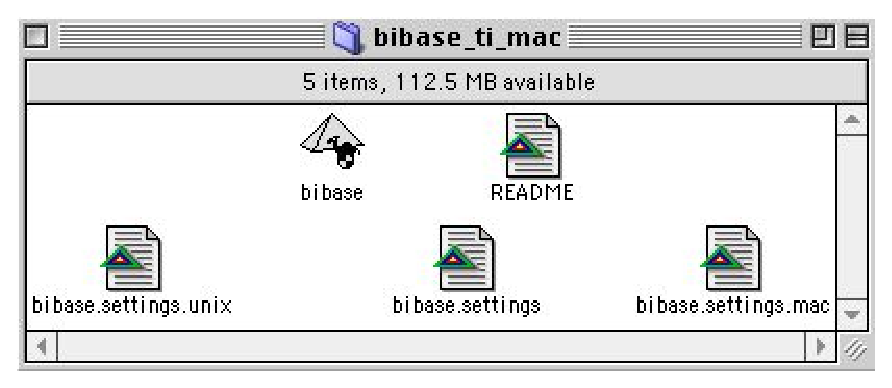
\epsfig{file=files.eps, width=100mm}}
\caption{The distribution.}
\label{fig:files}
\end{figure}
These are all of the files that you need to get going (initially) 
with Bibase.  There is the binary for Bibase, the README file (which 
you might as well since it asks so nicely), and three settings files: 
bibase.settings, bibase.settings.mac and bibase.settings.unix.  The 
first of these files is the settings file that specifies some initial 
bits and pieces for your version of bibase.  If you have a look in 
the bibase.settings file you will find (currently) three lines:
\begin{verbatim}
dbfilepath = 
bibfilename = bibase.bib
dbfilename = bibase.db
\end{verbatim}
These are the default settings for Bibase.  

The {\tt dbfilepath} 
variable is currently set to the directory that Bibase (i.e. the binary 
for the Mac version) is in.  You can use this to change the directory 
that the two database files {\tt bibase.bib} and {\tt bibase.db} are 
kept.  One known problem with this though is that it doesn't support 
spaces in file paths.  If you have a look inside either the 
bibase.settings.mac or the bibase.settings.unix files you will find 
where I have my files on both MacOS and Unix.  Note that on the Mac 
the directory separator is a colon (:) and on Unix the separator is a 
slash (/).  Also note that the settings file is the only bit that is 
system dependent, and even then only dependent upon directory 
separator.  The only reason I have included the files 
bibase.settings.mac and bibase.settings.unix is to show you how to set 
up the paths for these two operating systems.  

The {\tt bibfilename} variable is the name that you want to call your 
\emph{.bib} file.  This is the file that you will call in to BibTeX when 
writing your thesis or journal papers or whatever.  I have called mine 
\emph{bibase.bib} and this is also the default setting, you may call 
it whatever you like, so long as its extension is \emph{.bib}.  For 
example, if you are writing a thesis and are only interested in using 
Bibase for the time that you are writing up then you may wish to call 
the file \emph{thesis.bib} or something.  If you are using Bibase 
more long term then you may want to call it something else.  The known 
difficulty is that you can't have whitespace in the filename.

The {\tt dbfilename} is the name of the file used in the search 
engine.  This file is ``compiled'' from the \emph{.bib} file and it 
might be handy to keep it the same sort of name as the \emph{.bib} 
file.  I will refer to this file as the \emph{.db} file due to its 
default extension, but you can call it whatever you want.  Again, 
don't put whitespace in the filename otherwise things won't work.

As a final note in this section Mac users may find it handy to make an 
alias to Bibase and put it on 
your desktop or somewhere useful for easy access.  On Unix one should 
make a symbolic link to the bibase.pl file in your bibase directory 
from your bin directory and make the bibase.pl file executable.  If 
you don't understand all of that, don't worry too much at this stage 
as I will hopefully add an install script for the Unix version of 
Bibase.

\section{Main Menu}

When you start the application (either by typing ``bibase'' at the 
command line, or double clicking on the icon) you will see a window 
similar to \fig{fig:mainMenu}.  This is the {\bf Main Menu}.
\begin{figure}
\centerline{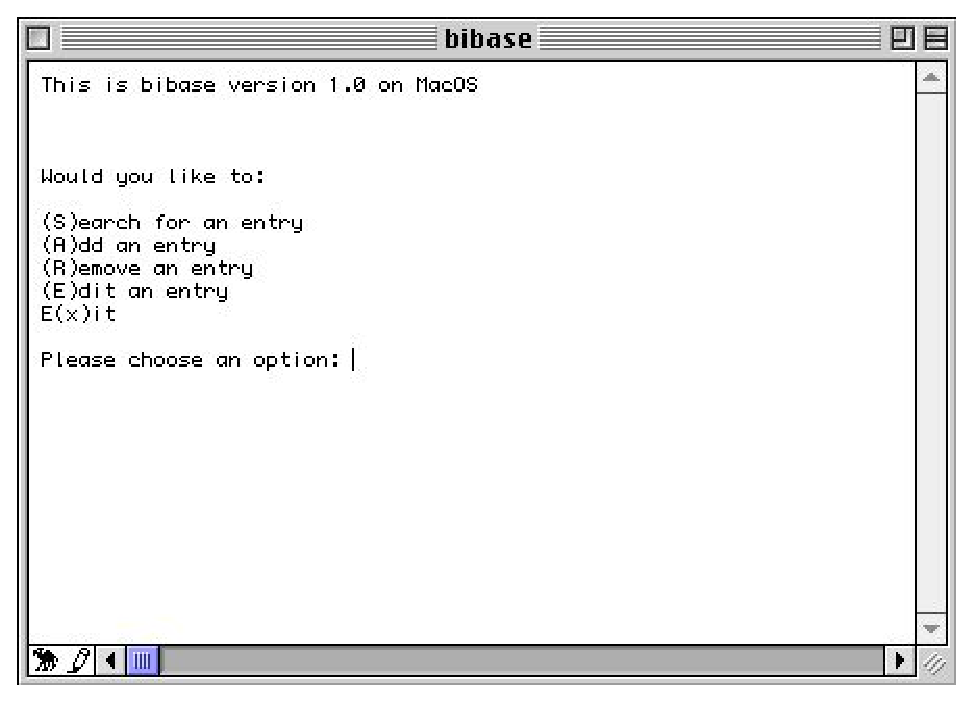
\epsfig{file=mainMenu.eps, width=100mm}}
\caption{Main menu.}
\label{fig:mainMenu}
\end{figure}
Not that it is particularly significant, but it is the entry point to 
the program.  From here we can do a few things, namely, we can search 
something that already exists in the database (the Search option), we 
can add a new entry into the database (the Add option), we can remove 
an existing database entry (the Remove option), we can edit an existing 
database entry (the edit
option) and finally, we can exit the 
program (the Exit option).  Each of the menu options will now be 
discussed in turn.

\section{Search menu option}

This option, fairly obviously, searches the database.  To search the database 
one merely
needs to enter `s', `S', `l' or `L'\footnote{The options `l' and `L' 
are included for historical reasons as this used to be called the 
``lookup'' menu option, but I decided that ``search'' was a far better 
name.} and then one is taken to the next menu: the 
search options menu.
\begin{figure}[!ht]
\centerline{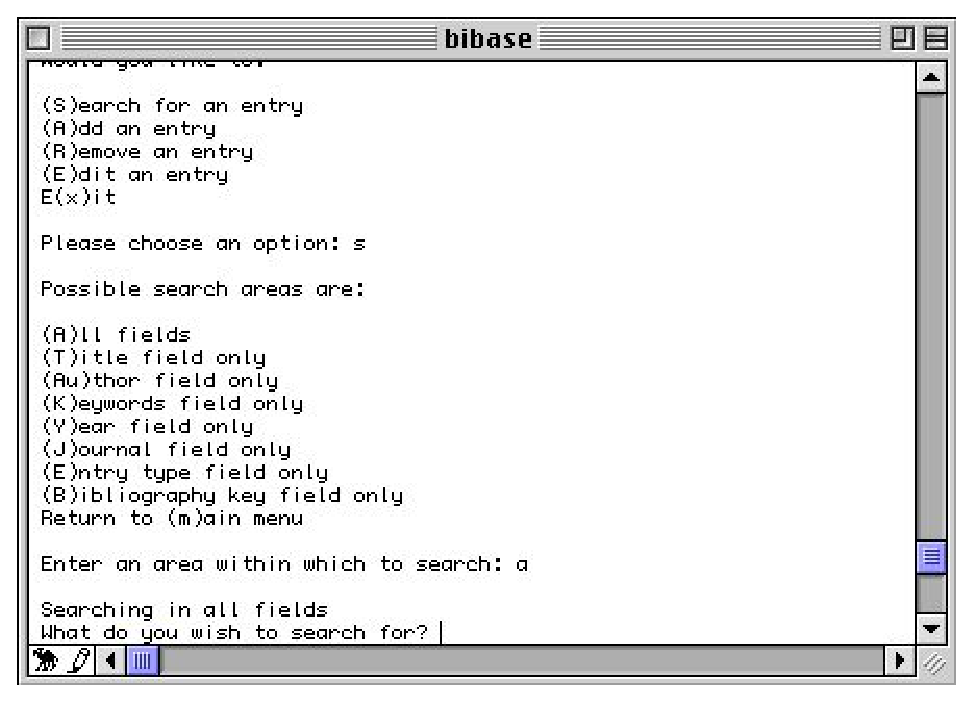
\epsfig{file=search.eps, width=100mm}}
\caption{Search menu.}
\label{fig:search}
\end{figure}
From here one can choose to either search in all fields available, or 
one from a selection of all possible fields.  These fields are: 
Title, Author, Keywords, Year, Journal, Entry type, and Bibliography 
key.

To choose to search only in the Title field, enter either `t' or `T'.  
To search only in the Author field, enter either `au', `AU' or `Au' 
(`aU' is also supported, but only for the case where someone makes a 
bit of a typo).  The remaining fields are entered in much the same 
way as shown in \fig{fig:search} by the letter with parentheses 
around it.

The Keywords, Entry type and Bibliography key fields may confuse some 
people, and I will explain what they are now.

The Keywords field is added for Bibase only.  BibTeX does not 
recognise the field, but nevertheless doesn't worry about the fact 
that it is superfluous for its own purposes.  The Keywords field is 
included so that one can enter various keywords about a given paper 
so that one isn't limited by searching in only the author or title 
fields to find out what a paper is about.  Basically, the keywords 
field helps to characterise a paper better and provides more 
information which will hopefully be useful at some time in the future.

The Entry type field refers to the kind of entry one has made, for 
instance, it could be a journal article, hence it would be an entry of 
type Article, or perhaps a chapter in a book, and then it would be of 
type Chapter and so on, for more details of the other fields 
available in BibTeX, have a look in{\bf cite\{Lamport, Kopka and 
Daly\}}.  I have included the ability 
to search in the Entry type field just in case someone wants to see 
all entries that have type Book, say.  I don't expect this to be used 
too often, but it is included nonetheless.

The Bibliography key field is also known as the cite key field, since 
this is what one adds to the $\backslash$cite command in \LaTeX when 
referencing a paper or whatever.  I have shortened this in some 
places in the program to Bibkey and from now on will refer to it as 
the Bibkey field.  This field is added to aid more narrow kinds of 
searches and is based upon the way in which Bibase generates the 
Bibkey.  The Bibkey is generated by taking the last name of the first 
author of the work being entered, appending a year and then a number 
relating to how many entries there exist in the database by that 
author in that given year; each being separated by a colon.  The Bibkey 
is the argument given to the $\backslash$cite command.  For instance, if a 
journal article was written by J Bloggs (and possibly some others) in 1999 
and it was found to be the third such paper to be entered into the database, 
then the Bibkey would be generated as:  Bloggs:1999:3.  In adding 
this field to the searching possibilities I am hopefully taking care 
of the case when one thinks ``I know Bloggs published a paper on that 
sometime in 1999 -- I wonder which one it was''.  Hence, one merely 
needs to do a search in the Bibkey field using Bloggs:1999 as the 
search string and one will then find all papers with Bloggs as the 
first author during 1999.  This isn't as flexible as being able to 
search in the Author field and the Year field at the same time, but I 
will get around to that at some point in the future.

As an example of how to use the search engine, let's do a search in 
all fields.  We type `a' (or `A') at the prompt and are prompted for 
the search string like this:
\begin{figure}[!ht]
\centerline{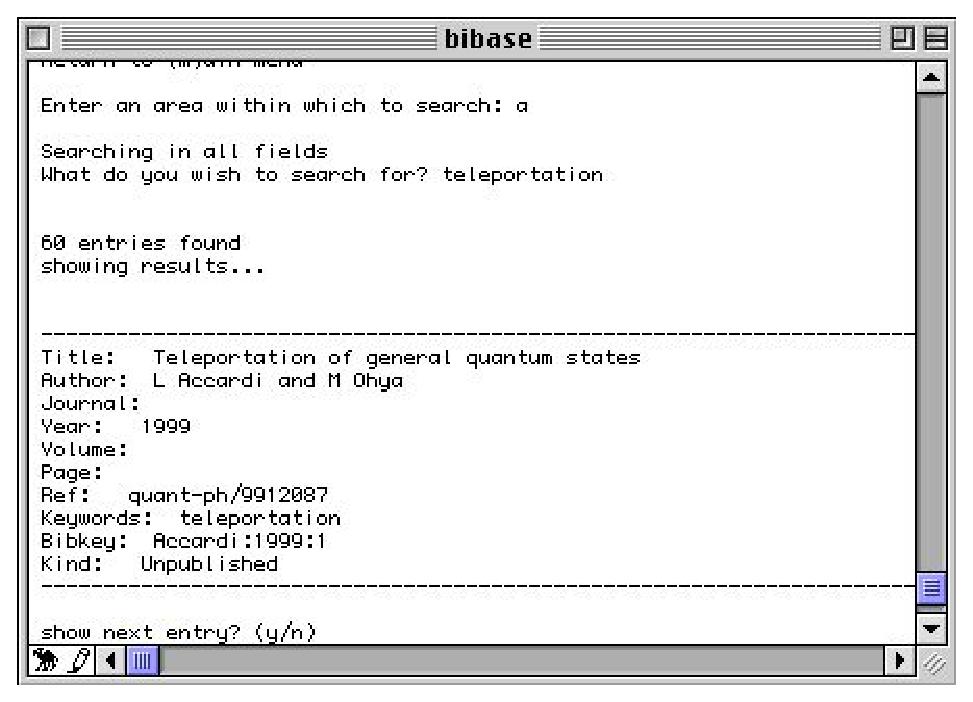
\epsfig{file=searchExample.eps, width=100mm}}
\caption{Searching in all fields.}
\label{fig:searchExample}
\end{figure}
We are then reminded that we are searching in all fields and are then 
prompted with the phrase {\tt What do you wish to search for?}.  In 
this case we are searching for the keyword {\tt teleportation}.  
Bibase then tells us how many entries match the query and immediately 
lists the first entry.  What you see here is a standard output format and 
not specific for the particular kind of entry, hence this 
\emph{Unpublished} entry doesn't show the {\tt Journal:}, {\tt Volume:} 
or {\tt Page:} fields.

We are then prompted if we wish to see the next entry to which the 
answer to the affirmative can be either `Y', `y' or just a carriage 
return (i.e. just hit the return key).  The answer to the negative 
can be either `N' or `n', after which the {\bf Main Menu} reappears.

\section{Add menu option}

The add menu will probably be the one that you use the most, 
especially in the initial stages when you are first making your 
database of papers, books, theses etc.  One selects the add menu by 
typing `A' or `a' and then the return key, the screen should look 
like \fig{fig:addEntry}.
\begin{figure}[!ht]
\centerline{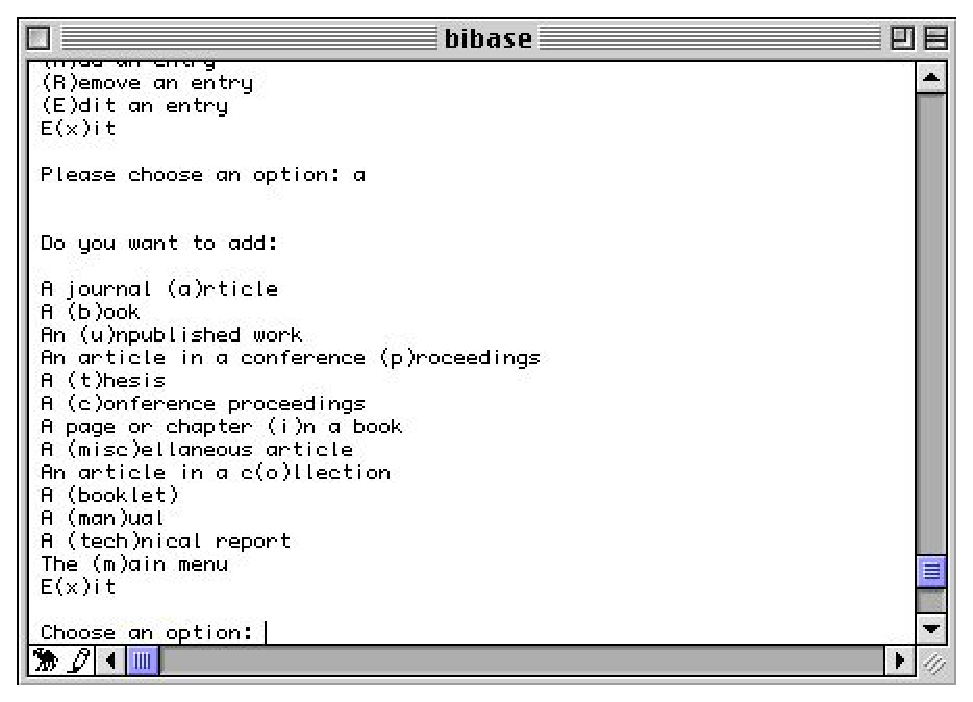
\epsfig{file=addEntry.eps, width=100mm}}
\caption{Adding an entry.}
\label{fig:addEntry}
\end{figure}
I have added into this menu all fields that the Emacs editor 
specifies in its BibTeX mode, which will hopefully suffice most 
users.  In my own work (I'm a PhD student in Physics) I have added 
over 300 journal articles, books, etc. and haven't needed any other 
fields (as yet), so hopefully this will be the same for you.  One can 
add 12 different kinds of entry into the database, from a journal 
article to a technical report to an unpublished work (such as those 
found on preprint archives like {\tt http://xxx.lanl.gov}).  The 
various entry types can be selected by typing the string of letters 
(or just the letter in most cases) that are enclosed in parentheses.  
One can also go back to the main menu from here (by choosing `m' or 
`M') or one can exit the program entirely (more on this option later).

Let's choose to add a journal article; the entry of a bogus article 
is outlined in \fig{fig:addArticleFull}.  We are prompted with {\tt 
Choose an option:} and select `a'.  We are then reminded that we are 
adding a journal article, just in case this wasn't what you want to 
do.  If you didn't want to add an article merely hit return at the 
{\tt Title:} prompt without entering anything into the field and you 
will be taken back to the add menu.  Some of these fields are needed 
by BibTeX, so if you don't add anything into the field then you will 
be shown an error message and taken back to the add menu.  This is 
also a feature, as if one makes a mistake, but realises that it was on 
the previous line and so one can't go back to fix the error directly, 
one can ``add nothing'' to a compulsory field and get back to the add 
menu to start again.  This saves having to complete your entering and 
then go to the edit menu to edit the mistake.  In the journal article 
entry type the {\tt Title:}, {\tt Author(s):}, {\tt Journal:}, {\tt 
Year:} and {\tt Keywords:} fields are required (the {\tt Keywords:} 
field is required by Bibase, not by BibTeX). 

The data entered into \fig{fig:addArticleFull} shows some of the 
``features'' of Bibase.  
\begin{figure}[!ht]
\centerline{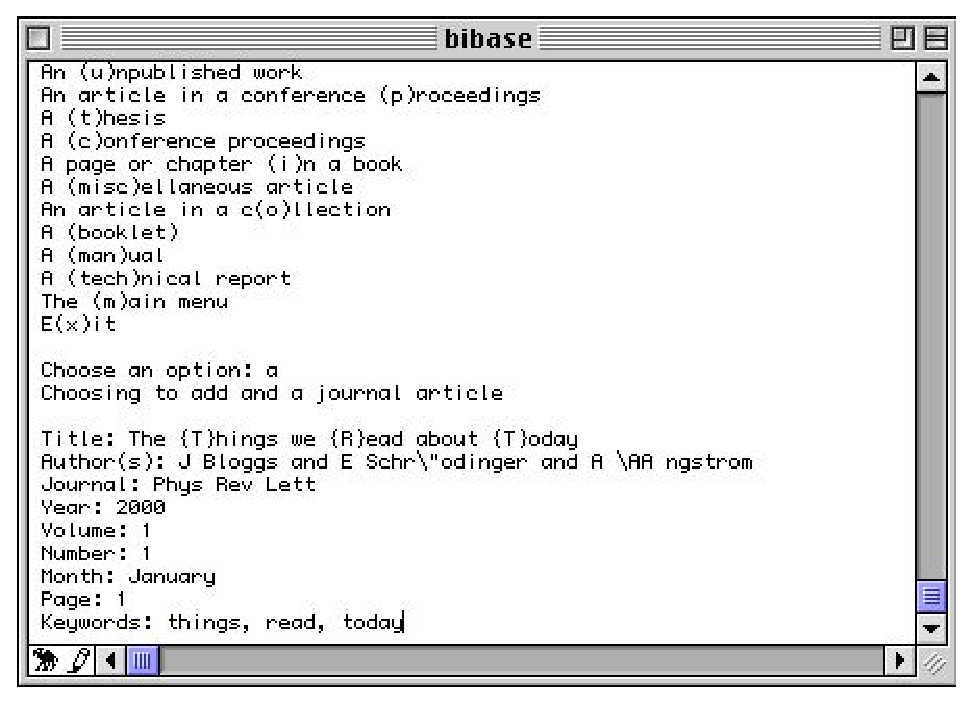
\epsfig{file=addArticleFull.eps, width=100mm}}
\caption{Entering data into an article template.}
\label{fig:addArticleFull}
\end{figure}
For instance, if one wants to retain 
capitals in things like titles one must put braces around the letters 
as necessary (BibTeX makes the title look the way it wants it in 
BibTeX's output, so it needs to be told if you want it to look 
otherwise).  As \LaTeX can handle many kinds of symbols and accents 
you can add these into the fields in Bibase as you would if you were 
using \LaTeX or BibTeX directly.  The {\tt Author(s):} field shows 
this with umlauts shown above the `o' in Schr\"odinger and the circle 
above the `A' in \AA ngstrom.  The problem with this ``feature'' is 
that when it comes to searching the database you need to specify 
\begin{verbatim}
Schr\"odinger
\end{verbatim}
to get a match.  You also need to add the space in 
\begin{verbatim}
\AA ngstrom
\end{verbatim}
which is a bit of a pain at times, but it fits with \LaTeX.  

One should realise that we are entering data almost directly into the 
fields of ``raw'' BibTeX in Bibase, the program is just a handy way to 
do that, so that sort of explains some of these ``features''.  

The {\tt Author(s):} field needs some special mention.  The last name 
of the first author can't have any special symbols added to it 
otherwise the Bibkey (otherwise known as the cite key) won't be 
generated correctly.  There may be ways around this, without being 
too politically incorrect.  For instance, German names can alter the 
umlaut by adding an `e' so that Schr\"odinger becomes Schroedinger.  
Unfortunately, if no other alternative exists you may just have to 
enter the name as written and be a bit politically incorrect.

There is one more point to make about the {\tt Author(s):} field.  
{\bf All} authors must be separated with the word `and'.  This is a 
BibTeX feature, and remember when I said before that you are really 
entering ``raw'' BibTeX, just in a nice way, well that's why.

The {\tt Volume:}, {\tt Number:}, {\tt Month:} and {\tt Page:} fields 
are all optional, and if you don't want to add anything here, don't.  
Just hit the return key and go to the next field.  However, the {\tt 
Keywords:} field is compulsory, but only for Bibase, and it can be 
delimited in any fashion you like, it is just a bit of extra 
functionality that I found handy, but for some reason I wanted it 
compulsory.

As mentioned above, one can exit directly from this menu as seen in 
\fig{fig:exitFromAdd}.
\begin{figure}[!ht]
\centerline{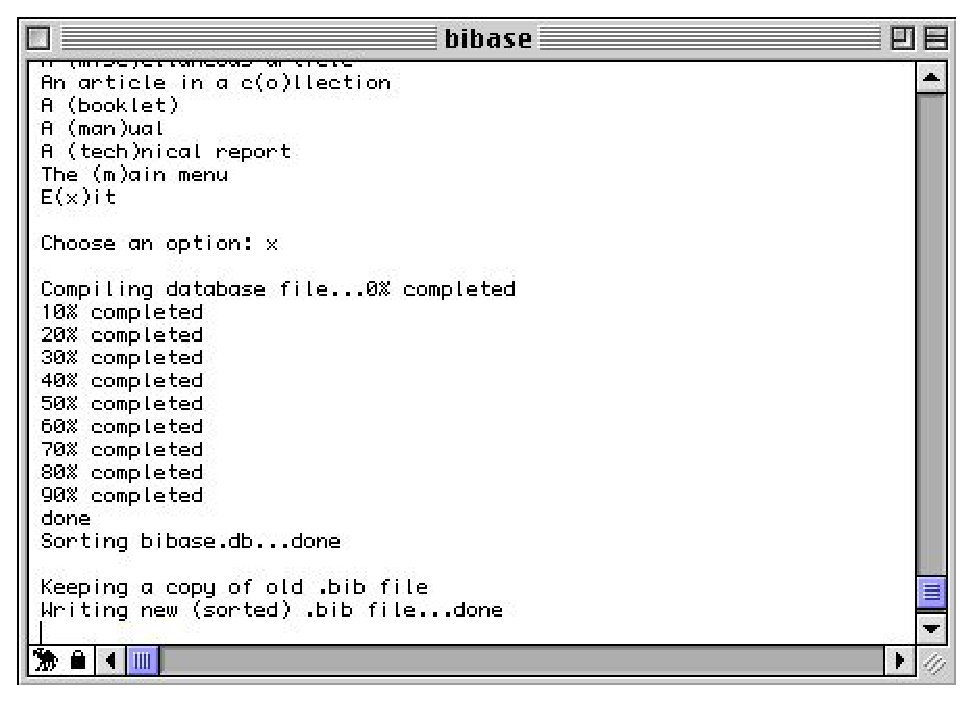
\epsfig{file=exitFromAdd.eps, width=100mm}}
\caption{Exiting from the add menu.}
\label{fig:exitFromAdd}
\end{figure}
If one has entered data into the database, Bibase checks to see if the 
main database (the \emph{.bib} file) has been modified and then 
``compiles'' the \emph{.db} file so that when you want to search, the 
new data is included in the search.  The ``compilation'' can take a 
while on oldish systems (I use a PowerBook 1400) so I added an update 
of the compilation process by showing how much of the 
\emph{.bib} file has been processed; on 500MHz Linux box it happens 
almost instantaneously.  Bibase does some other stuff 
(fairly obviously, from the output) but it isn't really necessary to 
understand what is going on here, other than it is my way of making a 
system independent sort for the \emph{.bib} file.

\section{Remove menu option}

By selecting either `r' or `R' from the main menu one can choose to 
remove an entry.  By doing so, we see the menu in \fig{fig:remove}.
\begin{figure}[!ht]
\centerline{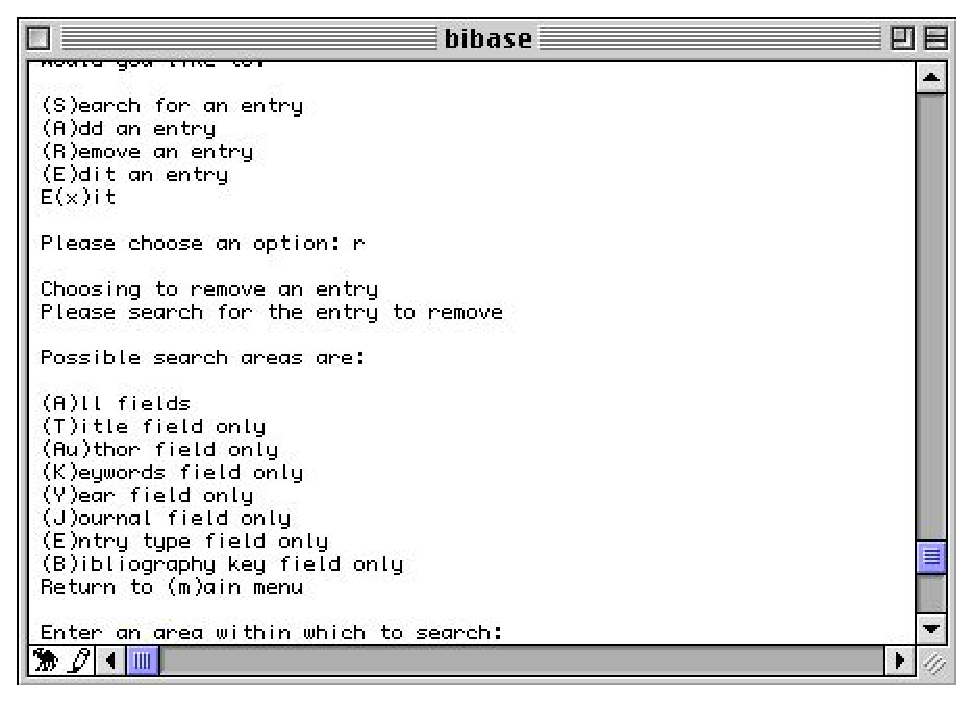
\epsfig{file=remove.eps, width=100mm}}
\caption{Removing an entry.}
\label{fig:remove}
\end{figure}
In this menu we have to search for the entry that we wish to remove, 
so we get a menu the same as for an ordinary search.  Again, we can 
search in a variety of fields to limit as much as possible the number 
of hits we get in the search.  Let's search in the {\tt Author} field 
for the name {\tt Bloggs} that we have just added to the database.  In 
doing so we get the output in \fig{fig:searchToRemove}.
\begin{figure}[!ht]
\centerline{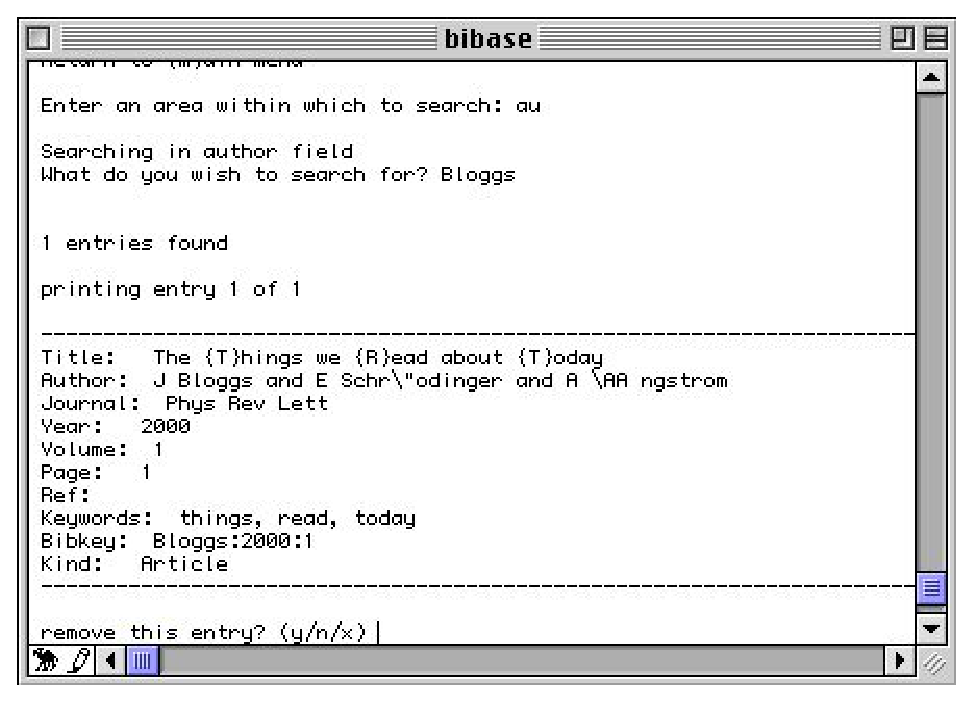
\epsfig{file=searchToRemove.eps, width=100mm}}
\caption{Searching to remove an entry.}
\label{fig:searchToRemove}
\end{figure}
We are then prompted with: {\tt remove this entry? (y/n/x)}.  The 
possible responses are `y', `Y' for yes, we do want to remove this 
entry.  `N', `n' or just hitting the return key will take you to the 
next entry (if there are any more, in this case there aren't), and 
pressing either `x', `X', `q', `Q', `m' or `M' will take you back to 
the main menu.  If there are no more entries then choosing the ``no'' 
option will also take you back to the main menu.  In this case we 
want to get rid of this entry so we choose the option `y' and get the 
output in \fig{fig:removeFinish}.
\begin{figure}[!ht]
\centerline{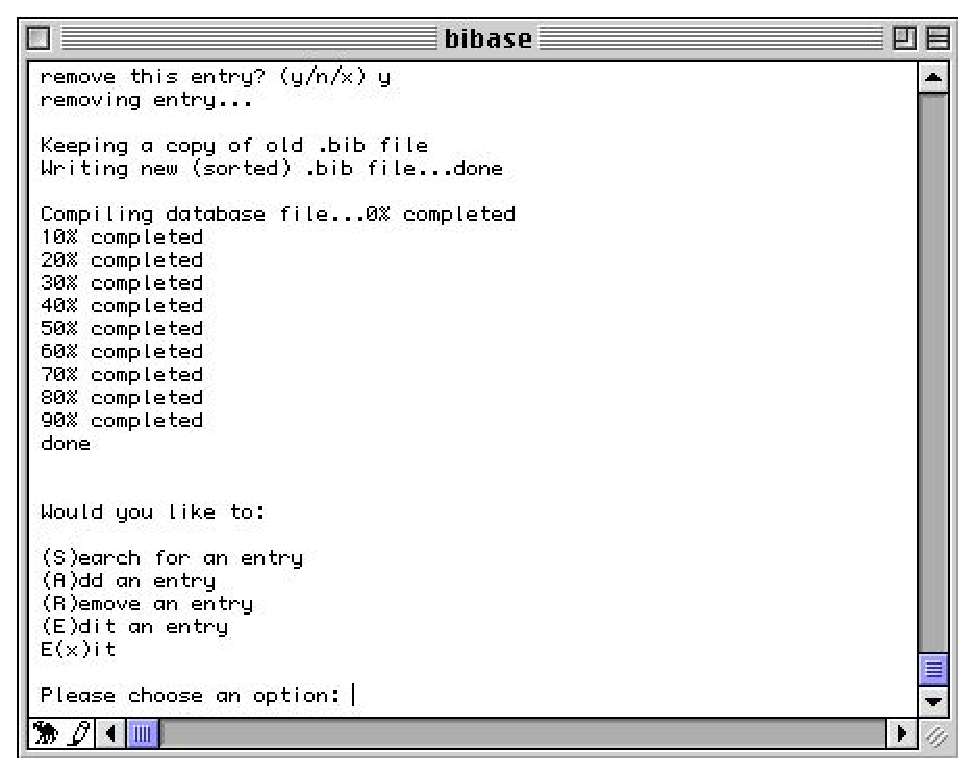
\epsfig{file=removeFinish.eps, width=100mm}}
\caption{Completing a remove operation.}
\label{fig:removeFinish}
\end{figure}
We are told what the program is doing so that we can be happy that it 
is doing what it is supposed to be doing.  It first removes the entry 
from the \emph{.db} file and then writes a new (sorted) \emph{.bib} 
file from which a new \emph{.db} file is ``compiled'' so that 
searching can be done correctly.  We are then taken back to the main 
menu.

\section{Edit menu option}

Editing entries in the database requires you to do a few things, so I 
will try and explain everything as carefully (and possibly as 
verbosely) as I can. 

To edit an entry one must choose edit from the main menu, search for the 
correct entry, select the relevant entry, select the relevant field 
to edit, edit (replace really) the field, verify that the field is 
correct and then either edit another field or return to the main 
menu.  This may sound like a lot to do, but I have just been very 
detailed in my explanation, and really there isn't that much to do, 
as Bibase guides you as best as it can through each stage.  Let's go 
through an example.  We start by selecting edit from the main menu (we 
enter either `e' or `E').
\begin{figure}[!ht]
\centerline{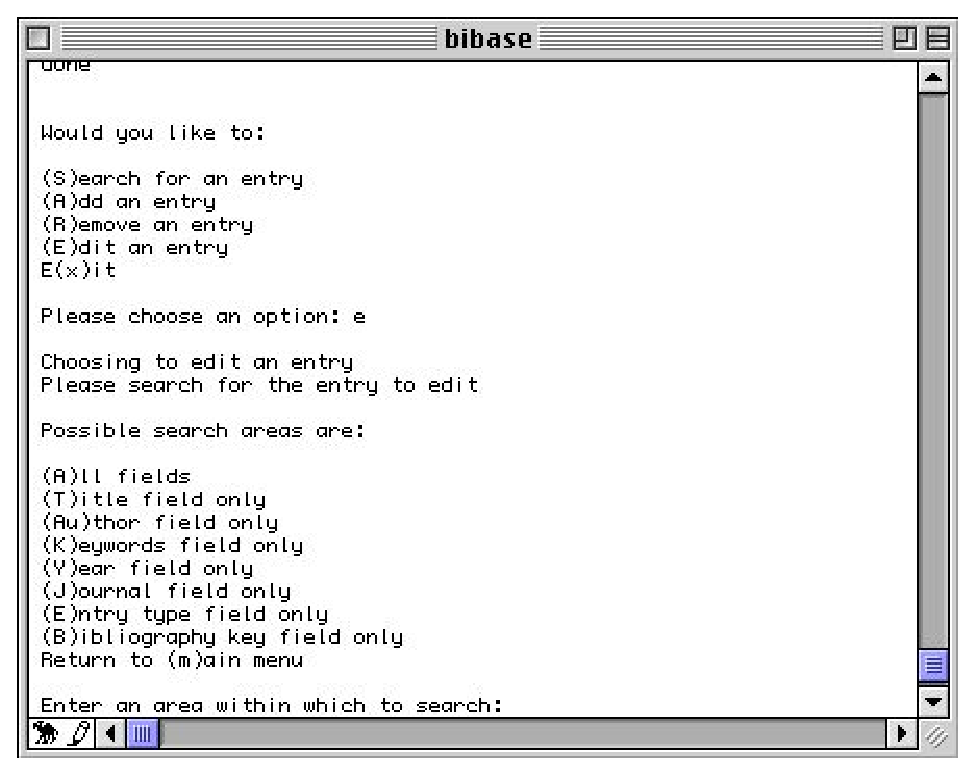
\epsfig{file=edit.eps, width=100mm}}
\caption{Editing an entry.}
\label{fig:edit}
\end{figure}
Now we are prompted to search for an entry to edit, note that this is 
the same as searching for an entry normally, so if you don't know how 
to do that then read the section on searching above.  We choose to 
search in the title file and we search for ``teleportation'' (one of 
my main areas of research).  
\begin{figure}[!ht]
\centerline{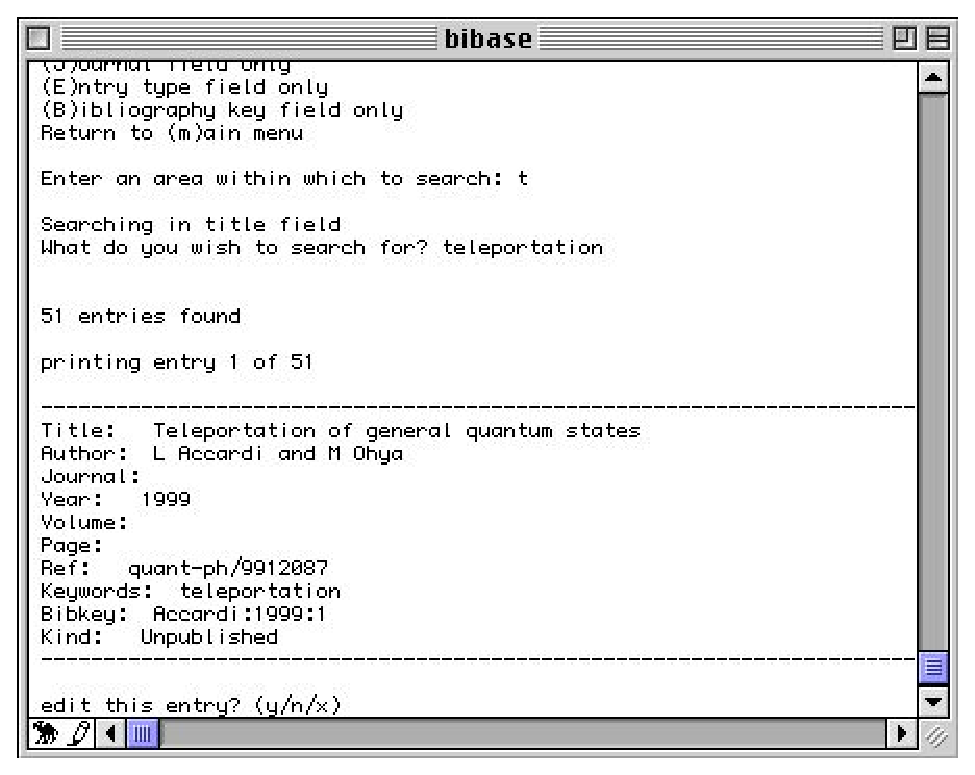
\epsfig{file=searchToEdit.eps, width=100mm}}
\caption{Searching to edit an entry.}
\label{fig:searchToEdit}
\end{figure}
We are told that 51 entries have been found in the title field, are 
shown the first entry and are prompted as to whether or not we want 
to edit this entry.  As in removing an entry we have three options as 
to what to do, we can choose to edit the entry by entering `y' or 
`Y', we can choose not to edit the entry by entering either `n', `N' 
or just hitting the return key and we are then shown the next entry in 
the search, or we can choose to enter `x', `X', `q', `Q', `m' or `M', 
in either case we are taken back to the main menu.

We choose to edit the current entry by selecting `y' and pressing 
return, \fig{fig:editTitle} shows this.
\begin{figure}[!ht]
\centerline{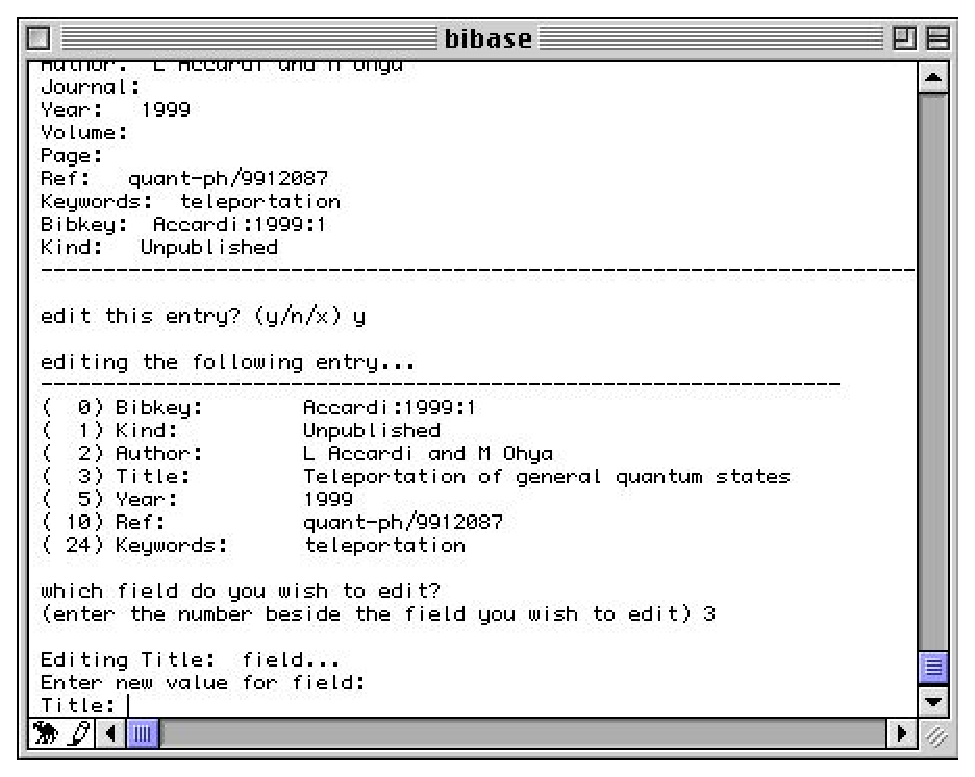
\epsfig{file=editTitle.eps, width=100mm}}
\caption{Editing a Title entry.}
\label{fig:editTitle}
\end{figure}
Bibase now shows you all of the fields that are present in this 
particular entry and the name of each field.  Each field is also 
referenced by a number to the left of each field name in parentheses.  
Now Bibase prompts us to ask which field we want to edit, in this case 
we want to edit the {\tt Title:} field and we see that the number to 
the left of it in parentheses is 3 so we enter this at the prompt.  
Bibase now tells us which field we have selected to edit and now 
prompts us for the new value for the field.  We change the title to 
read as that shown in \fig{fig:editCheck}.
\begin{figure}[!ht]
\centerline{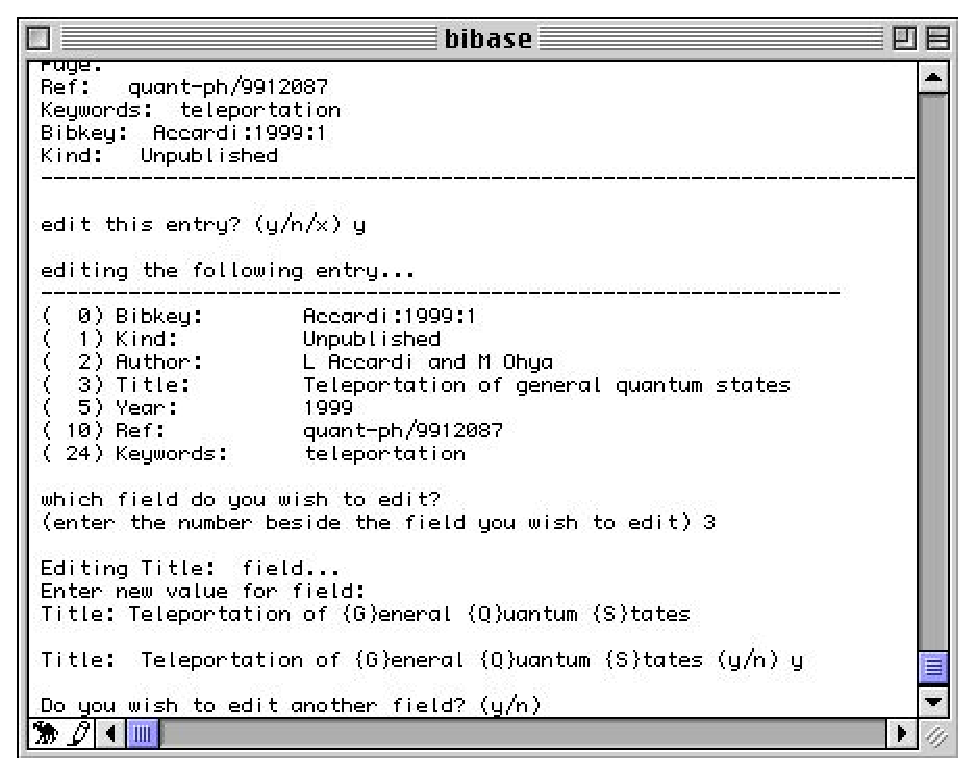
\epsfig{file=editCheck.eps, width=100mm}}
\caption{Entering and checking the new title entry.}
\label{fig:editCheck}
\end{figure}
Upon hitting return after entering in the new field value we are shown 
the new value of the field and asked if this is correct by Bibase 
merely echoing the new field value and adding {\tt (y/n)} after it.  
Not helpful I know, but I guess I will get around to making it 
prettier one day.  Bibase now asks if you wish to edit another field, 
in this case we don't want to so we select `n' and hit return.  If, 
however, you did want to edit another field, you merely choose `y' 
or 'Y'' and the output shown in \fig{fig:editTitle} is shown again for 
you to choose another field to edit.  After selecting `n' (or `N') 
Bibase does a sort and ``compilation'' so that if you want to search 
once you get back to the main menu you can do so with the correct 
entries in the database.  I have shown this here in 
\fig{fig:editFinish}.
\begin{figure}[!ht]
\centerline{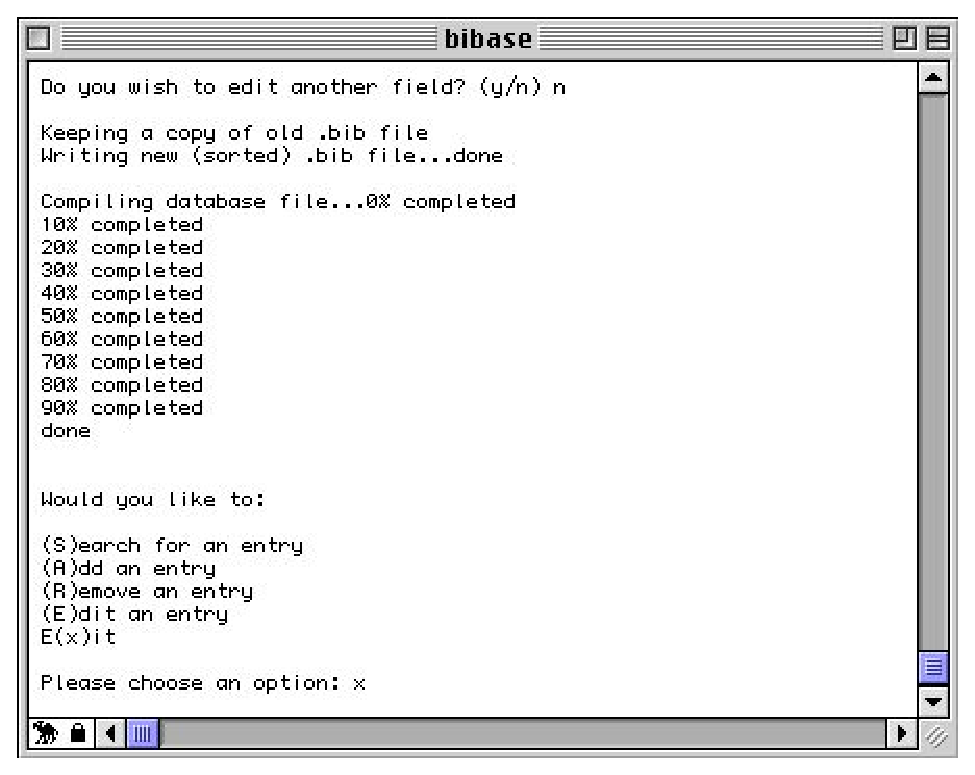
\epsfig{file=editFinish.eps, width=100mm}}
\caption{Finishing an edit operation.}
\label{fig:editFinish}
\end{figure}

\section{Exit menu option}

Choosing `x', `X', `q' or `Q' from the main menu exits you from the 
program in much the same way as you can see in \fig{fig:editFinish}.  
What happens here isn't all that interesting, but so that you know, if 
you have only added new entries to the database, then Bibase will do a 
``compilation'' and sort and rewrite so that everything is hunky dory 
before you leave the program.  Notice that a copy is kept of the old 
\emph{.bib} file just in case 
something stuffed up and you want to get your last (and hopefully 
correct) data back.
If there is no need to compile (as in 
\fig{fig:editFinish} or if you have only done a search or something 
that doesn't require compilation) then the program will just exit.  On 
Unix systems you will be taken back to the system prompt and it will 
be very obvious that you will have exited Bibase.  On Macintosh it is 
not so obvious that you have finished as it looks as though Bibase is 
just sitting there ``looking'' at you.  It has, however, finished, you 
just need to choose ``Quit'' from the file menu or press Cmd-Q on the 
keyboard.  One way to tell if Bibase is still going on Macintosh is to 
look in the bottom left-hand corner of the window.  There you will 
see a little camel and beside that a closed padlock icon (see 
\fig{fig:editFinish}), this means 
that you have exited the program and just need to quit the binary 
that is still running (maybe I will work out how to shut it down 
properly one day but at present it doesn't really seem to matter that 
much).  You will notice that in all figures other than 
\fig{fig:editFinish} the little camel has a ``writing pencil'' icon 
beside it, this means that the program is still running, so there is 
definitely a way to check to see if things are still going or not.

\chapter{Graphical User Interface Version}

This is a bit behind in its development (as well as the 
documentation), so once the program is satisfactory then I will write 
some docs.

\chapter{Interfacing Bibase with BibTeX}

Okay, we now have a \emph{.bib} file and a \emph{.db} file.  What do I 
do with them?  And where does BibTeX fit in?  Well, to answer these 
two questions read on.  

You don't need the \emph{.db} file at all to be able to interface 
with BibTeX, it is only needed for Bibase for searching purposes.  You 
will, however, need the \emph{.bib} file for use with BibTeX.  How you 
use the file varies very slightly with what you are doing, there is a 
standard way to include the \emph{.bib} file, but how the output from 
BibTeX is used can vary if you are writing a paper for a journal or if 
you are writing a book or a thesis.  The simplest of these to explain 
is for a book or thesis so I will explain this first.

\section{Bibase, BibTeX, books and theses}

To use BibTeX, have a look in either {\bf cite\{Lamport, Kopka and 
Daly\}} or the BibTeX documentation which probably came with your 
\LaTeX distribution.  I will give a bit of an idea of what to do 
here.  

In writing your thesis or book you are probably using the \emph{book} 
class file (or something like it), so your \LaTeX source file 
probably looks something like this:
\begin{verbatim}
\documentclass[12pt,a4paper]{book}

this is the preamble

\begin{document}

\title{J Bloggs}
\date{\today}
other sundry commands...
\maketitle

\frontmatter
\tableofcontents
\tableoffigures

\mainmatter

\chapter{Blah blah}

blah blah blah (etc)

\end{document}
\end{verbatim}
So how do you change this to add the ability to add citations easily?  
There are a couple of ways to do this (I just thought you should know 
that there are other ways to do it) but since this is really just for 
BibTeX I'll only explain that here.

Okay, you need a \emph{.bib} file (yay! we have that thanks to 
Bibase!) and then have to add a couple of extra commands into your 
\LaTeX file to be able to reference the entries in the \emph{.bib} 
file.  You do this by putting 
\begin{verbatim}
\bibliography{/some/path/or/other/bibase}
\end{verbatim}
in your \LaTeX file where you want the bibliography entries to appear.
Notice that one can put in either the full path to the \emph{.bib} 
file or a relative path (i.e. by putting 
{\tt ../../texthings/thesis/bibase}).  Also note that there is no 
extension to the \emph{.bib} filename, \LaTeX and BibTeX know that it 
should have a \emph{.bib} extension, so you don't have to add it.  

You then add the line
\begin{verbatim}
\bibliographystyle{<style>}
\end{verbatim}
so that BibTeX knows which bibliography style file to use.  Just 
enter the kind of style where I have put {\tt <style>} above.  One 
can use styles of ``plain'', ``unsrt'' or ``apsrev'' among 
others\footnote{For instance, the ``unsrt'' style puts the citations 
in order of appearance in your \emph{.tex} file, and adds bold and 
italics as necessary, the ``apsrev'' style file puts the output into 
a format acceptable for publication in the American Physical Society 
journals such as Physical Review Letters etc.}.

Now, to cite references in your database you only need to type in 
\begin{verbatim}
\cite{<bibkey>}
\end{verbatim}
when you want to add a reference,
where {\tt <bibkey>} is the cite key (or Bibkey as I have called it) 
that appears in your \emph{.bib} file database.  This will point to 
all of the information necessary to output and properly format your 
bibliographic entries.

To get everything to work you then have to run \LaTeX over your 
source (i.e. \emph{.tex}) file then run BibTeX, and then run \LaTeX 
{\bf twice} (this makes sure that all of the cross-references are 
correct) and then your document ``should'' have a references section 
with nicely formatted entries.  This all may sound complicated and a 
lot of work, but it is easier than entering in all of your 
bibliography entries every time you want to add a new citation and 
then make sure that you are entering it in the correct format for your 
supervisor or the journal you are publishing in or whatever.  Put 
plainly there is a lot of ``donkey work'' that BibTeX can do for you 
so you might as well use it.

\section{Bibase, BibTeX and Papers}

When writing a paper for a publication in a journal (such as the 
Physical Review) you follow the instructions in the previous section 
for adding bibliographic citations to your documents using BibTeX.  
You will, however, need to do a little more work when it comes to 
final submission of the paper.  Initially, you can just use your 
\emph{.bib} database and give your most recent version to colleagues 
who you may be writing the paper with, so that they can ``TeX up'' 
your document with all of the relevant references.  But notice that 
you probably won't be using all of the references that appear in your 
database for your paper (please don't be silly and write a new 
\emph{.bib} file for each paper, this is a LOT of extra work and part 
of the reason why I 
wrote Bibase in the first place, so you can have just the one file 
that does a lot of hard, boring work for you).  The extra bit of work 
comes when you are finally ready to submit your preprint (I am 
assuming in electronic form) to either directly to the journal or to 
some preprint archive.  These places really don't want to see all of 
the journals you have collected so please, don't include your 
\emph{.bib} file when you submit, but do the following first.  You 
will note that BibTeX leaves a file with extension \emph{.bbl} in 
your working directory (it ``should'' be in the same place as the 
\emph{.tex} file and other ``dot'' files).  This file is what you 
would have had to have written by hand yourself, but BibTeX has been 
nice enough to generate for you.  Go to this file, select the whole 
file and copy it into your main \emph{.tex} document where you have 
the {\tt bibliography} command.  Now, comment out the {\tt 
bibliography} command by putting a percentage sign (\%) in front of 
it.  Save the \emph{.tex} file and rerun it through \LaTeX so that 
everything still works.  If everything is as it was before and all of 
the references are nicely formatted and in the right order (if not, 
then consult either a local guru and/or a text such as {\bf 
cite\{Lamport, Kopka\}}) then you are finally ready to submit (don't 
stop sweating though, as if you have already published before this is 
when you {\bf start} sweating about your paper, not when you {\bf 
stop} ;-).

I am pretty sure that is all you need to know for that part, if you 
are publishing (and especially if you are publishing for the first 
time) good luck!  And don't stress too much, referees \emph{can} be nice 
people!  :-)

\chapter{Concluding remarks}

Well, that is basically all there is to know about Bibase.  I hope 
you find it useful, and if not useful then at least a reasonably 
handy.  Please remember that this software is postcardware, so if you 
can please send me a postcard from where you are from, or where you 
are (you can say a brief hello too if you want, and maybe what you 
think about my program).  The address to send postcards to is 
\begin{verbatim}

Paul Cochrane
Physics Department
University of Queensland
St. Lucia
QLD 4072
AUSTRALIA

\end{verbatim}
so yeah, if you feel like it and if you like what I have done drop me 
a line!

If you got this far in the docs then thanks for reading this far!  
You have done well!

Best of luck with your BibTeX-ing and Bibase-ing!

\end{document}